% !TEX root = thesis.tex
%\newcommand{\baselineEvalFigure}{
\begin{figure}[t]
    \centering
    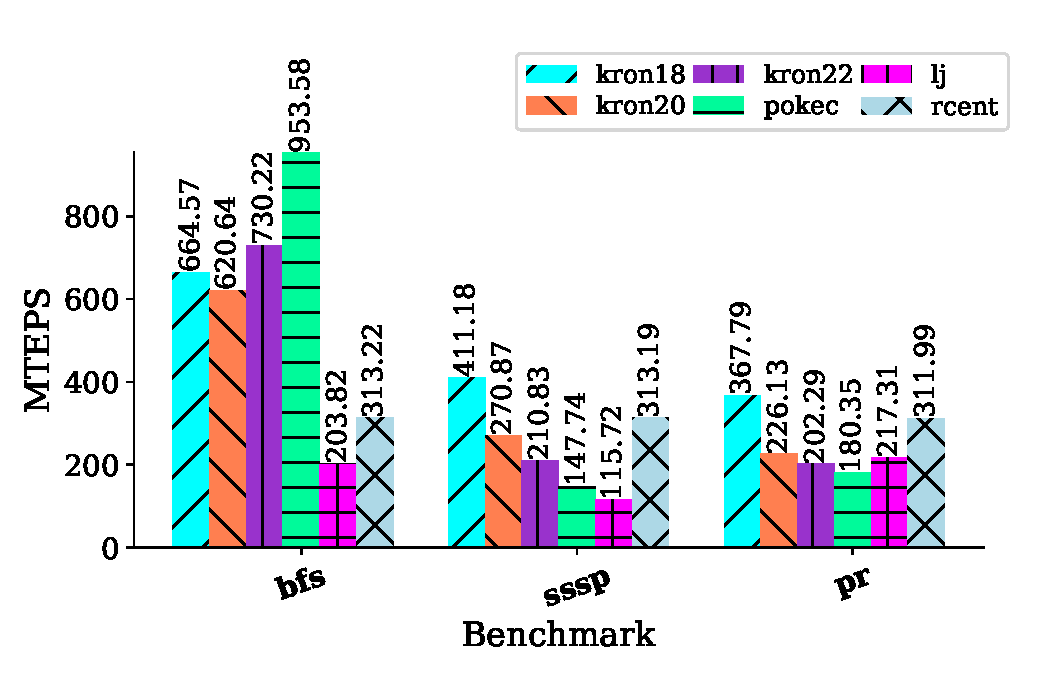
\includegraphics[scale = 0.5]{graphit-figures/baseline.pdf}
    \caption{Baseline code generation results for each benchmark in the dense pull direction with no manycore specific optimizations.}
    \label{pap:generals:sec:eval:fig:baseline}
\end{figure}
}

\newcommand{\pushEvalFigure}{
\begin{figure}[t]
    \centering
    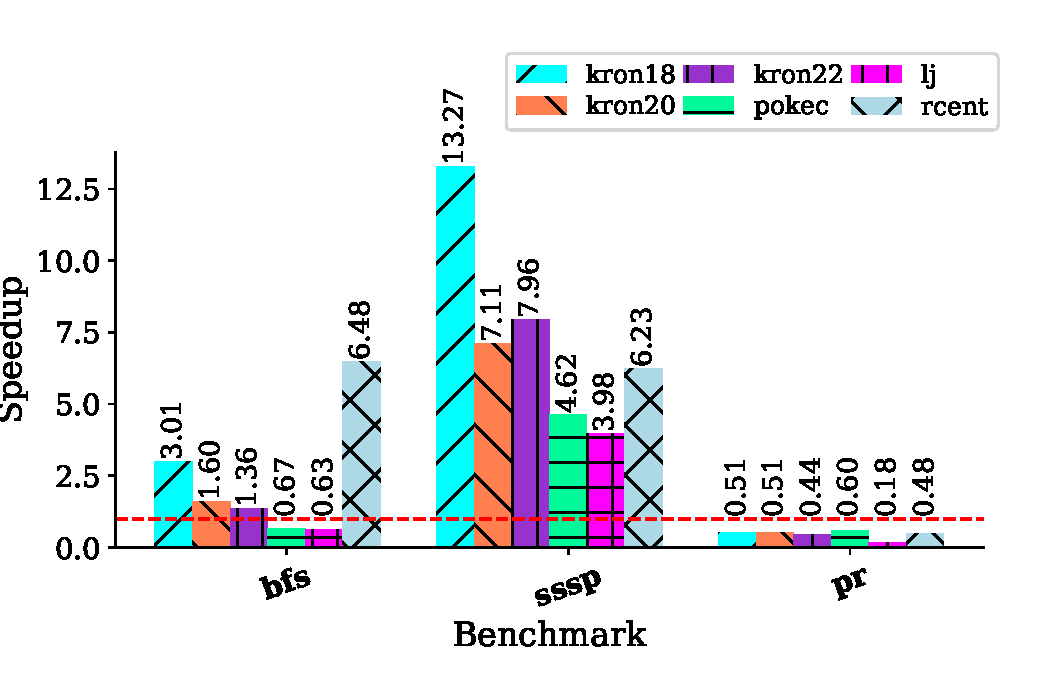
\includegraphics[scale = 0.5]{graphit-figures/push.pdf}
    \caption{Baseline code generation results for each benchmark in the push direction with no manycore specific optimizations.}
    \label{pap:generals:sec:eval:fig:push}
\end{figure}
}

\newcommand{\edgeSpeedupFigure}{
\begin{figure}[t]
    \centering
    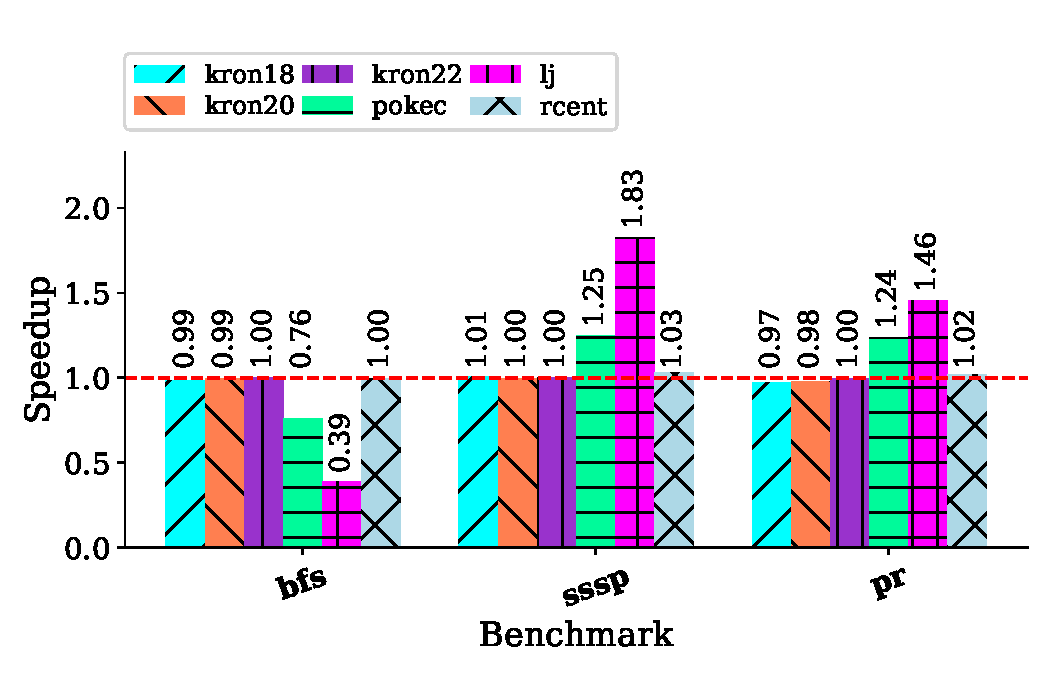
\includegraphics[scale = 0.5]{graphit-figures/edge.pdf}
    \caption{Speedup results for edge based optimization over the baseline dense pull implementation for each benchmark.}
    \label{pap:generals:sec:eval:fig:edge}
    \vspace{-2mm} 
\end{figure}
}

\newcommand{\blockBFSFigure}{
\begin{figure}[t]
    \centering
    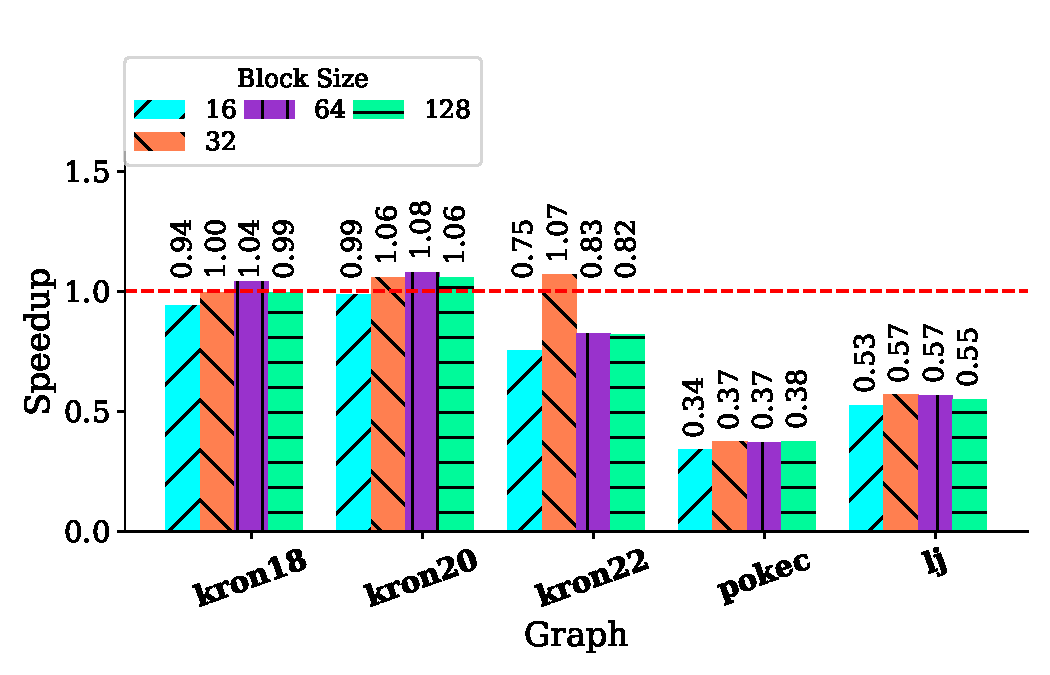
\includegraphics[scale = 0.5]{graphit-figures/bfs-block.pdf}
    \caption{MTEPS results for varying block sizes using the blocked access method on BFS.}
    \label{pap:generals:sec:eval:fig:bfsblock}
\end{figure}
}

\newcommand{\blockSSSPFigure}{
\begin{figure}[t]
    \centering
    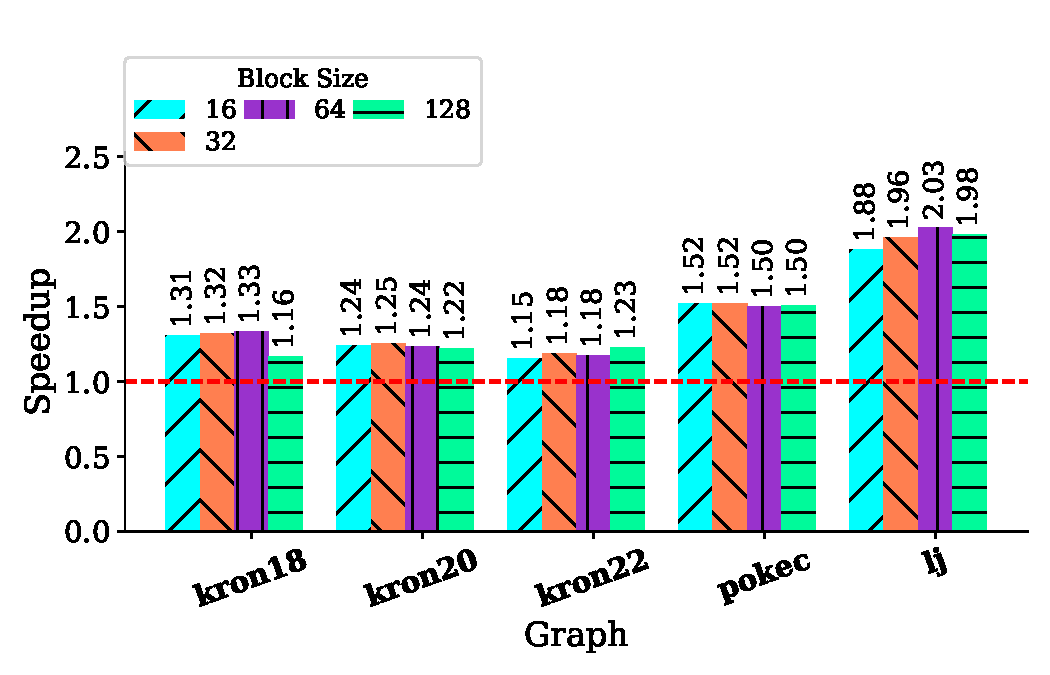
\includegraphics[scale=0.5]{graphit-figures/sssp-block.pdf}
    \caption{Speedup results for varying block sizes using the blocked access method on SSSP. Speedup is calculated over the baseline pull direction implementation.}
    \label{pap:generals:sec:eval:fig:ssspblock}
\end{figure}
}

\newcommand{\cacheBFSFigure}{
\begin{figure}[t]
    \centering
    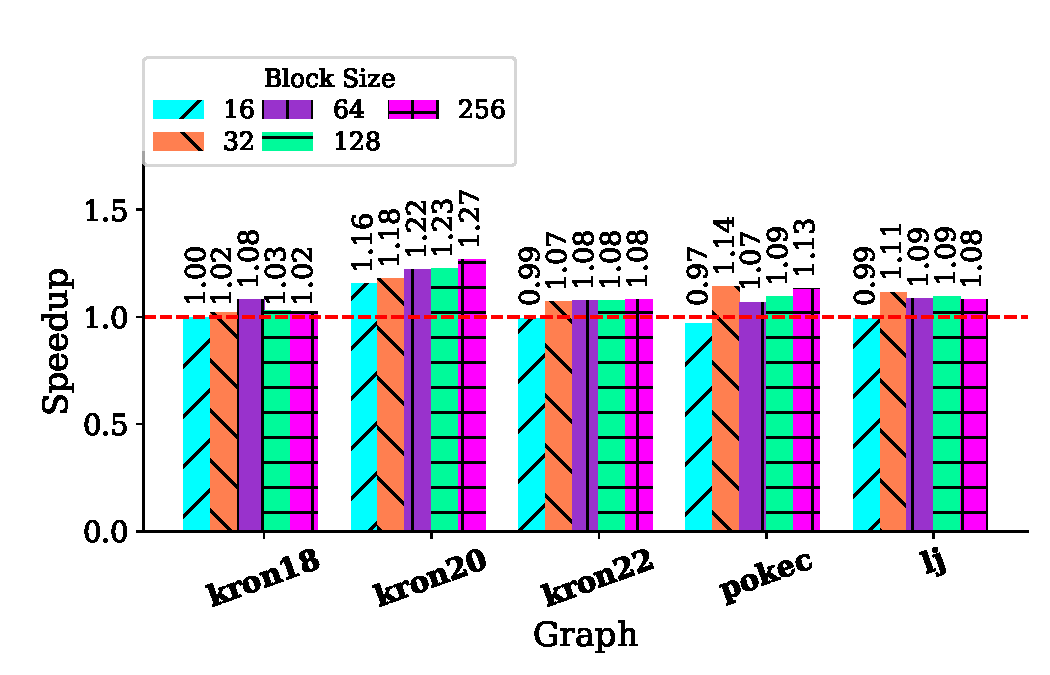
\includegraphics[scale = 0.5]{graphit-figures/bfs-cache.pdf}
    \caption{MTEPS results for varying work block sizes using the manycore aware vertex partitioning scheme on BFS.}
    \label{pap:generals:sec:eval:fig:bfscache}
\end{figure}
}

\newcommand{\cacheSSSPFigure}{
\begin{figure}[t]
    \centering
    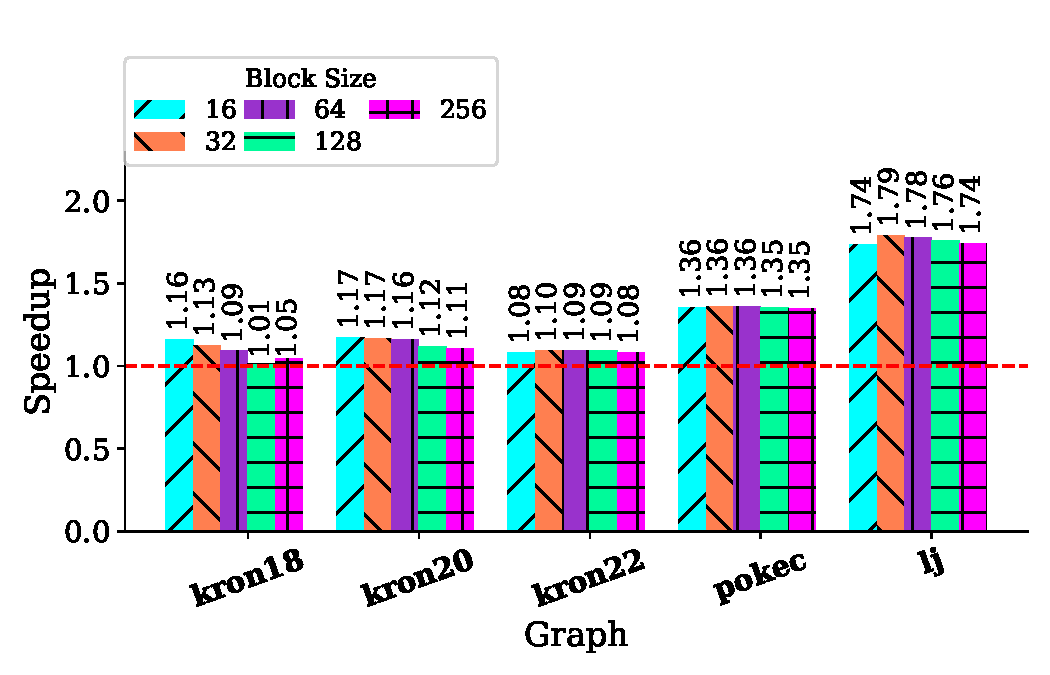
\includegraphics[scale=0.5]{graphit-figures/sssp-cache.pdf}
    \caption{Speedup results for varying work block sizes using the manycore aware vertex partitioning scheme on SSSP. Speedup is calculated over the baseline pull direction implementation.}
    \label{pap:generals:sec:eval:fig:ssspcache}
\end{figure}
}

\newcommand{\allBlockedFigure}{
\begin{figure}[t]
    \centering
    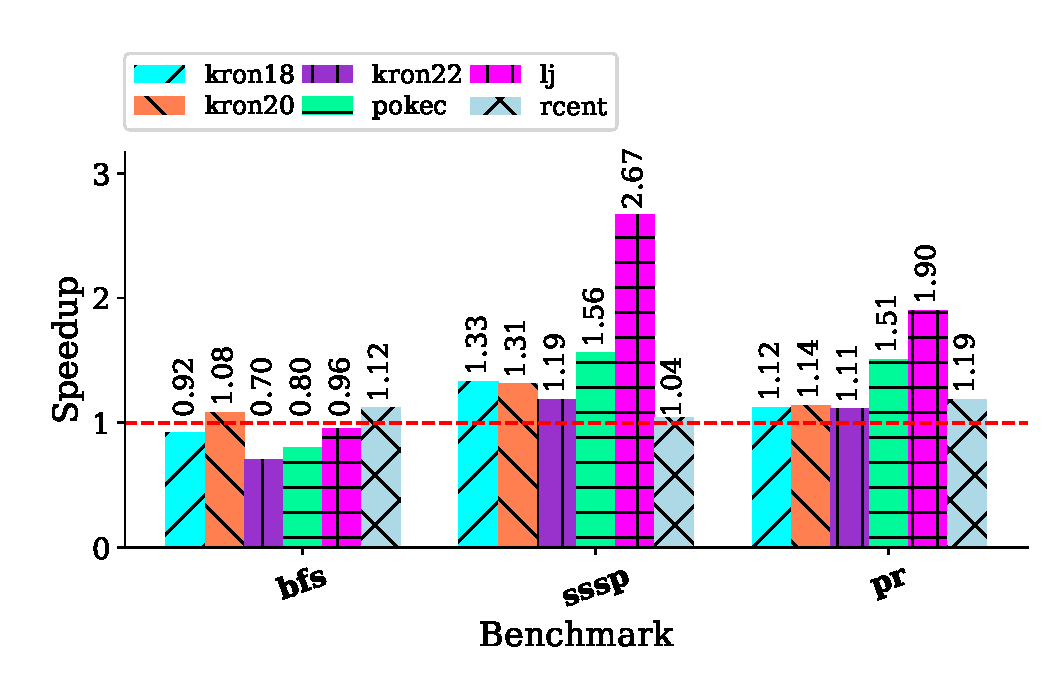
\includegraphics[scale = 0.5]{graphit-figures/all-blocked.pdf}
    \caption{Blocked access method speedup results for each benchmark. Speedup is calculated over the baseline pull direction implementation.} %For each graph and benchmark, block sizes of 16, 32, 64, and 128 elements were tested and the best performing block size is reported here.
    \label{pap:generals:sec:eval:fig:blocked}
\end{figure}
}

\newcommand{\allAlignedFigure}{
\begin{figure}[t]
    \centering
    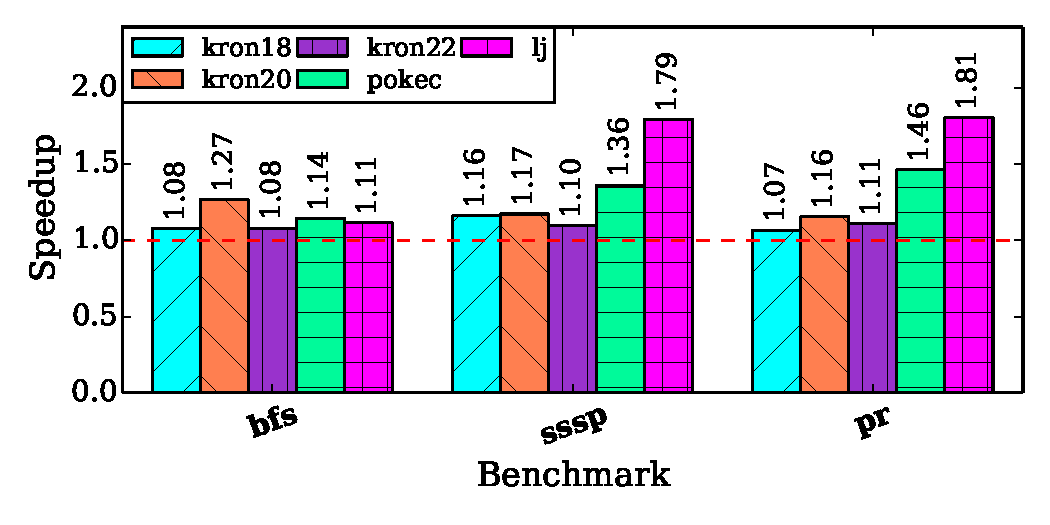
\includegraphics[scale = 0.5]{graphit-figures/align.pdf}
    \caption{Alignment-based partitioning speedup results for each benchmark. Speedup is calculated over the baseline pull direction implementation.} %For each graph and benchmark, work group sizes of 16, 32, 64, 128, and 256 vertices were tested and the best performing work group size is reported here.
    \label{pap:generals:sec:eval:fig:aligned}
    \vspace{-2mm} 
\end{figure}
}

%I am not sure if this is the best way to present an overview of results or if we need it. 
\newcommand{\overviewResultsTable}{
\begin{table}[]
\centering
\begin{tabular}{lrcl}
%\hline
\toprule
\textbf{Benchmark} & \textbf{Graph} & \textbf{MTEPS} & \textbf{Optimization} \\ \midrule
 \multirow{5}{*}{BFS}& kron18 & 457.09 & Cache-Aligned \pull \\ %\cline{2-4}
 & kron20 & 296.32 & Cache-Aligned \pull \\ %cline{2-4}
 & kron22 & 241.95 & Cache-Aligned \pull \\ %\cline{2-4}
 & pokec & 148.02 &  Cache-Aligned \pull\\ %\cline{2-4}
 & lj & 304.36 & Cache-Aligned \pull \\ \hline
 \multirow{5}{*}{PR}& kron18 & 412.34 & Blocked \pull \\ %\cline{2-4}
 & kron20 & 261.35 & Cache-Aligned \pull \\ %\cline{2-4}
 & kron22 & 224.88 & Blocked \pull \\ %\cline{2-4}
 & pokec & 272.57 & Blocked \pull \\ %\cline{2-4}
 & lj & 413.06 & Blocked \pull \\ \hline
 \multirow{5}{*}{SSSP}& kron18 & 467.08 & Cache-Aligned \pull \\ %\cline{2-4}
 & kron20 & 364.36& Baseline \push \\ %\cline{2-4}
 & kron22 & 404.27 & Baseline \push \\ %\cline{2-4}
 & pokec & 149.17 & Cache-Aligned \pull \\ %\cline{2-4}
 & lj & 268.87 & Cache-Aligned \pull \\ %\hline
 \bottomrule
\end{tabular}
\caption{Table containing best MTEPS results across all benchmarks and input graphs. The optimizations used to achieve these results are also listed above.}
\label{pap:generals:sec:eval:tab:overview}
\end{table}
}

\newcommand{\relatedMTEPSTable}{
\begin{table}[]
\centering
\begin{tabular}{cllll}
%\hline
\toprule
 \textbf{Source} & \textbf{Platform} & \textbf{Benchmark} & \textbf{Graph}  & \textbf{MTEPS} \\ \midrule
 \cite{slota2015high}& Xeon Phi MIC & CC & LJ (22) & 240 \\ %\hline
 \cite{slota2015high}& Xeon Phi MIC & CC & Flickr (19) & 140\\ %\hline
 %Galois \cite{aasawat2018well}& Ivy Bridge & PR & LJ (22) & 207.67 \\ \hline
 \cite{khorasani2014cusha} & GTX780 & BFS & LJ (22) & 272.4 \\ %\hline
 \cite{zhong2013medusa}& C2050 & BFS & KKT (21) & 351.5 \\ %\hline
 \cite{yang2019graphblast}& k40c & SSSP & LJ (22) & 334.2 \\ %\hline
 \cite{wang2016gunrock} & k40c & SSSP & LJ (22) & 217.9 \\
 \bottomrule

\end{tabular}
\caption{Performance results in MTEPS from other graph processing frameworks. The benchmark CC is strongly connected components.}
\label{sec:related:tab:mteps}
\vspace{-1mm} 
\end{table}
}
\newcommand{\graphInfoTable}{
\begin{table}[]
\centering
\begin{tabular}{c|c|c|c}
%\hline
 \textbf{Name} & \textbf{Scale} & \textbf{\# Vertices} & \textbf{\# Edges} \\ \hline %\hline
 kron18 & 18 & 262,144 & 4,194,304 \\ \hline
 kron20 & 20 & 1,048,576 & 16,777,216 \\ \hline
 kron22 & 22 & 4,194,304 & 67,108,864 \\ \hline
 pokec & 20.5 & 1,632,803 & 30,622,564 \\ \hline
 livejournal (lj) & 22 & 3,997,962 & 34,681,189 \\ %\hline
\end{tabular}

\caption{The vertex and edge information for each of the graphs used in our evaluation. We use synthetic \kron graphs used in the Graph500 benchmark and two real world graphs.}
\label{sec:eval:tab:graphs}
\end{table}
}
\newcommand{\tabHBParams}{
%\newcolumntype{D}{>{\raggedleft\arraybackslash}m{0.65in}}
%\newcolumntype{E}{>{\raggedright\arraybackslash}m{2.75in}}
\newcolumntype{D}{>{\raggedleft\arraybackslash}m{0.6175in}}
\newcolumntype{E}{>{\raggedright\arraybackslash}m{2.7175in}}
\begin{table}[h]
  \centering
  %\vspace{-0.1in}
  \resizebox{0.7\linewidth}{!}{
  \begin{footnotesize}
    \begin{tabular}{DE}
      \toprule
      \textbf{Cores} & 128 cores in a 16x8 grid \\
      & RISC-V 32-bit IMAF ISA @ 1 GHz\\
      & 4KB Instruction Cache \\
      & 4KB Data Scratchpad \\ %%[.5ex]
      \midrule
      \textbf{Cache} & 128KB Total Capacity \\
      & 32 Independent Cache Banks \\
      & 8-way Set Associative\\ [.2ex]
      \midrule
      \textbf{NoC} & Bidirectional 2D Mesh NoC (32-bit data, 64-bit address) \\ [.2ex]
      \midrule
      \textbf{Memory} & 2 HBM2 memory channels \\
      & 32 GB/s per channel \\
      & 512 MB per channel \\
      \bottomrule
    \end{tabular}
  \end{footnotesize}
  }
  \caption{Configuration of the HammerBlade manycore used in this evaluation.}
  \label{tab:hbParams}
\end{table}
}

\newcommand{\hbBlockingEvalTab}{
\begin{table}[h]
\centering
\begin{footnotesize}
\begin{tabular}{lccc}
\toprule
\textbf{Graph} & \textbf{DRAM Stalls} & \textbf{Bandwidth} &  \textbf{Speedup} \\ \midrule
LJ & 0.78 & 3.03 & 1.19    \\
HW &  0.79 & 2.17 & 1.53   \\
PC & 0.83 & 3.02 & 1.49     \\
\bottomrule
\end{tabular}
\end{footnotesize}
  \caption{Impact of the blocked access optimization on SSSP. Reduction in DRAM stalls, improvement in memory bandwidth utilization, and overall speedup. } %over the unoptimized version of \sssp. }%Results are shown for the three graphs for which the blocked access method was the optimal schedule.}
\label{tab:hb_blocking}
\end{table}
}

\newcommand{\edgeAwareHist}{
\begin{sidewaysfigure}
    \centering
    \subfloat[BFS 18]{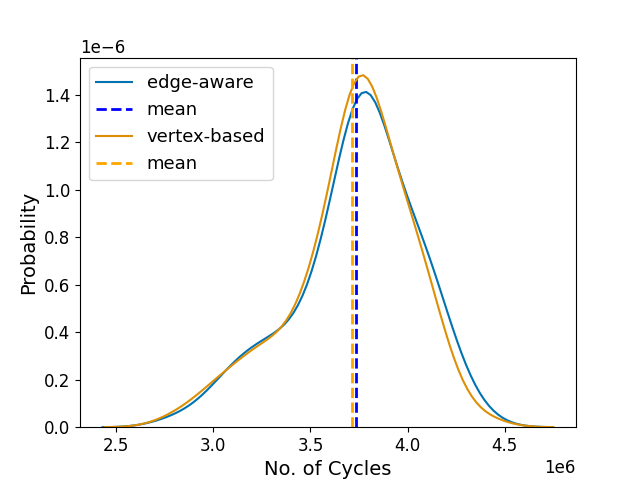
\includegraphics[width=0.3\textwidth]{graphit-figures/bfs-pull-18-edge-aware.png}}
    \subfloat[BFS 19]{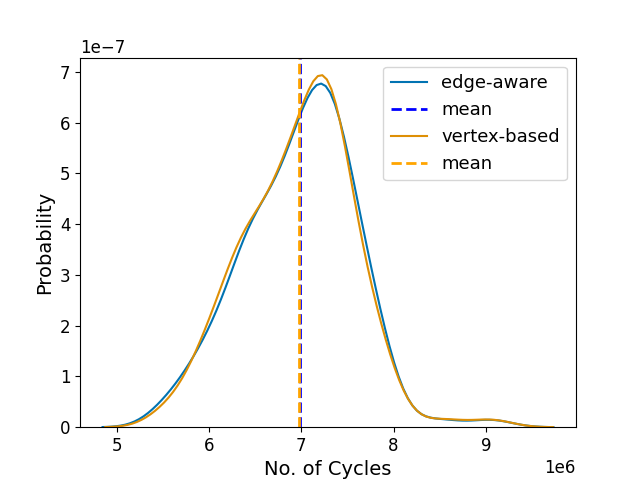
\includegraphics[width=0.3\textwidth]{graphit-figures/bfs-pull-19-edge-aware.png}}
    \subfloat[BFS 20]{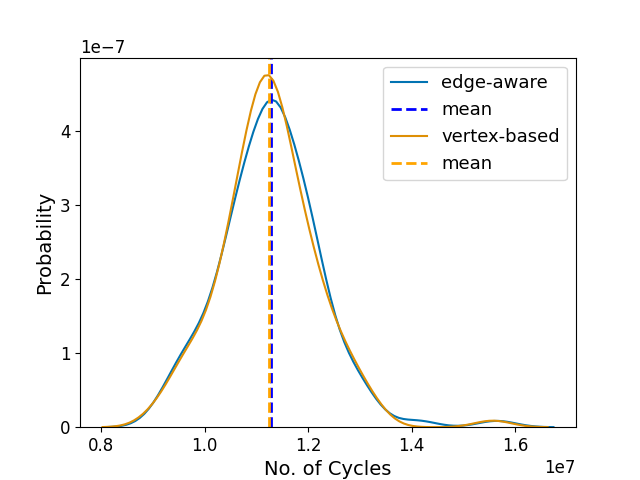
\includegraphics[width=0.3\textwidth]{graphit-figures/bfs-pull-20-edge-aware.png}} \\
    \subfloat[SSSP 18]{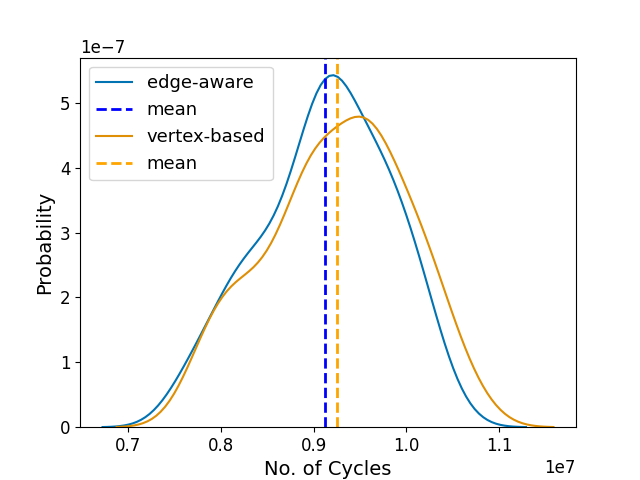
\includegraphics[width=0.3\textwidth]{graphit-figures/sssp-pull-18-edge-aware.png}}
    \subfloat[SSSP 19]{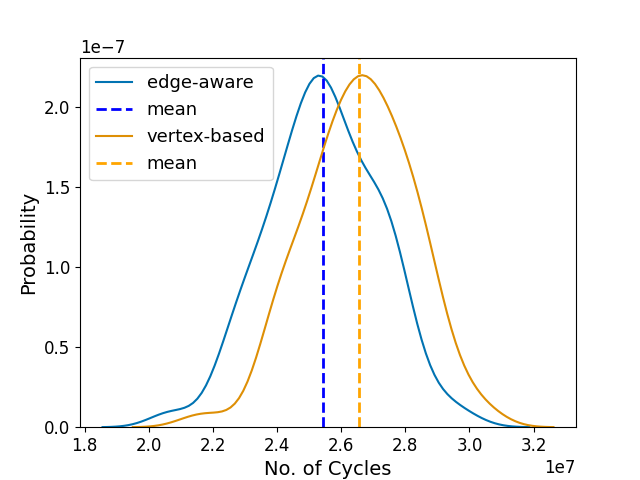
\includegraphics[width=0.3\textwidth]{graphit-figures/sssp-pull-19-edge-aware.png}}
    \subfloat[SSSP 20]{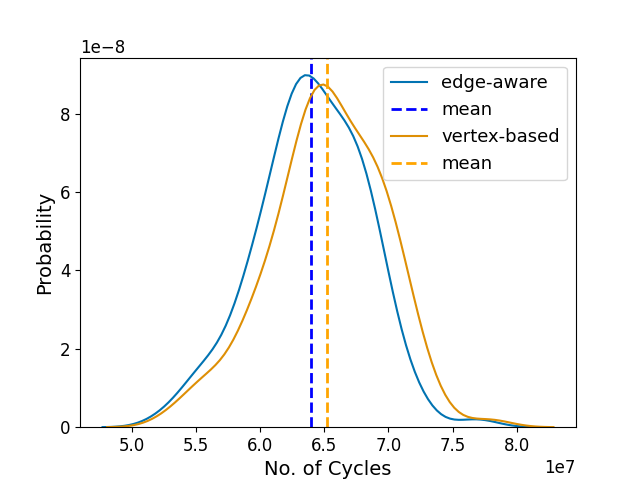
\includegraphics[width=0.3\textwidth]{graphit-figures/sssp-pull-20-edge-aware.png}} \\
    \subfloat[PR 18]{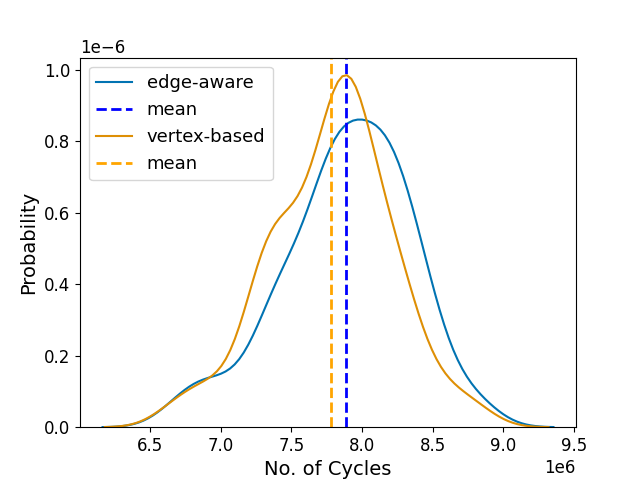
\includegraphics[width=0.3\textwidth]{graphit-figures/pr-pull-18-edge-aware.png}}
    \subfloat[PR 19]{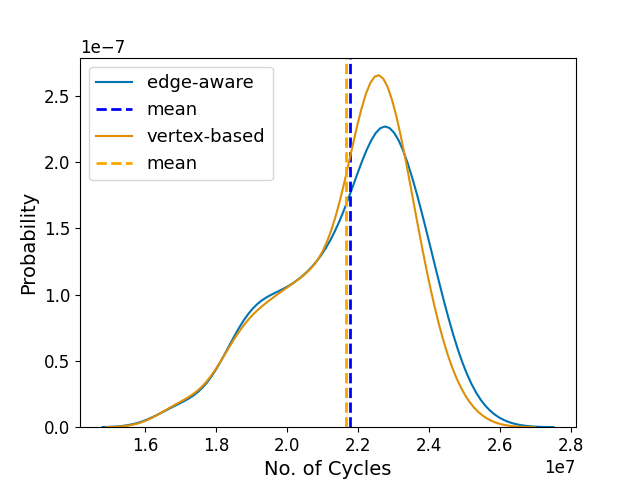
\includegraphics[width=0.3\textwidth]{graphit-figures/pr-pull-19-edge-aware.png}}
    \subfloat[PR 20]{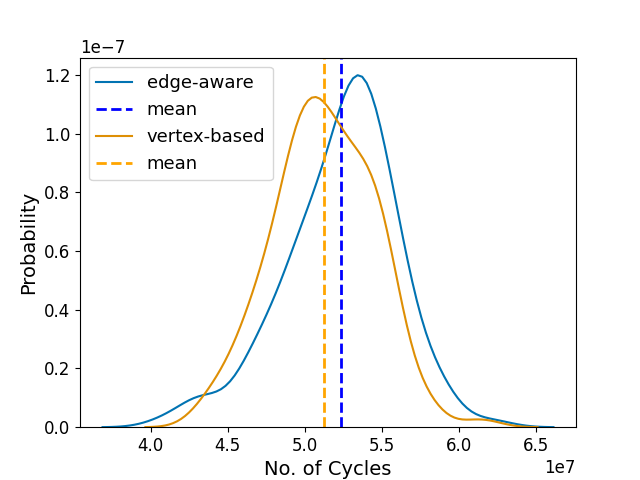
\includegraphics[width=0.3\textwidth]{graphit-figures/pr-pull-20-edge-aware.png}}
    \caption{Probability distribution of cycle counts for each core for vertex-based and edge-aware partitioning.}
    \label{fig:load_balance:cycledist}
\end{sidewaysfigure}
}

\newcommand{\alphatune}{
  \begin{figure}[h!]
    \centering
    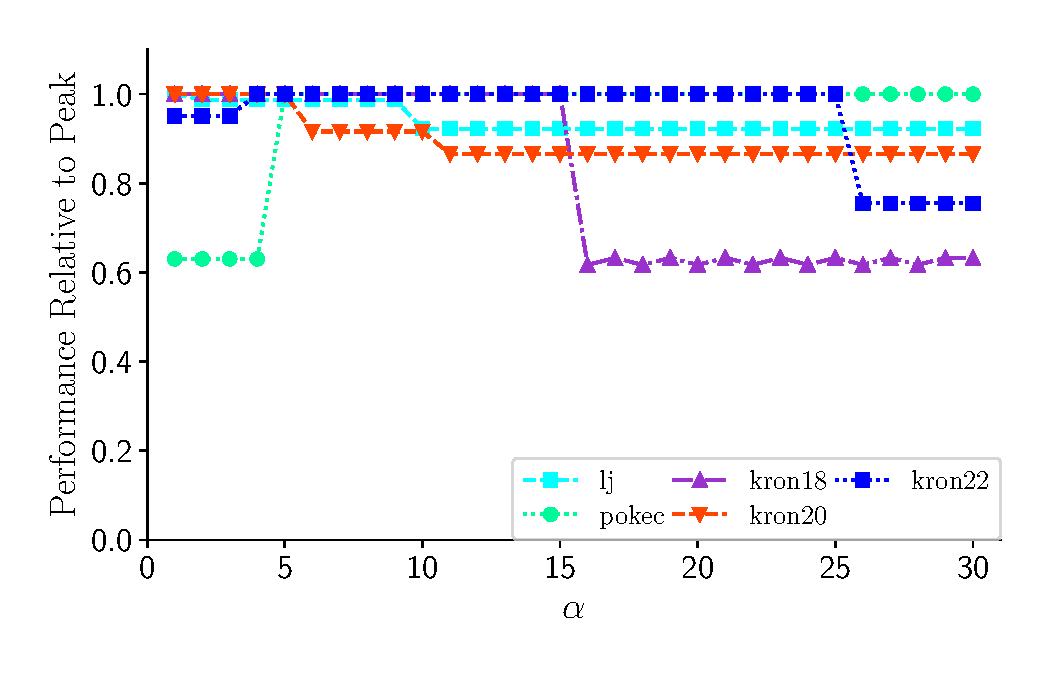
\includegraphics[scale=0.6]{graphit-figures/alpha.pdf}
    \caption{Results for tuning $\alpha$ on \hb. \todo{finish caption}}
    \label{fig:alpha_tuning}
  \end{figure}
}

\newcommand{\betatune}{
  \begin{figure}[h!]
    \centering
    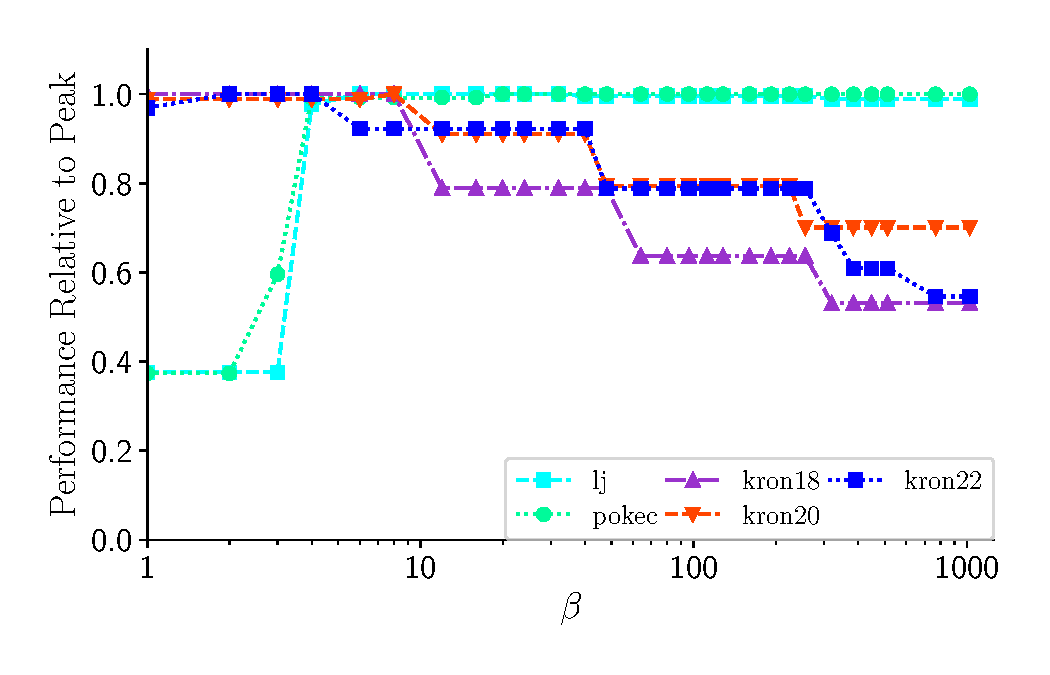
\includegraphics[scale=0.6]{graphit-figures/beta.pdf}
    \caption{Results for tuning $\beta$ on \hb. \todo{finish caption}}
    \label{fig:beta_tuning}
  \end{figure}
}

\newcommand{\hybridresults}{
  \begin{figure}[h!]
    \centering
    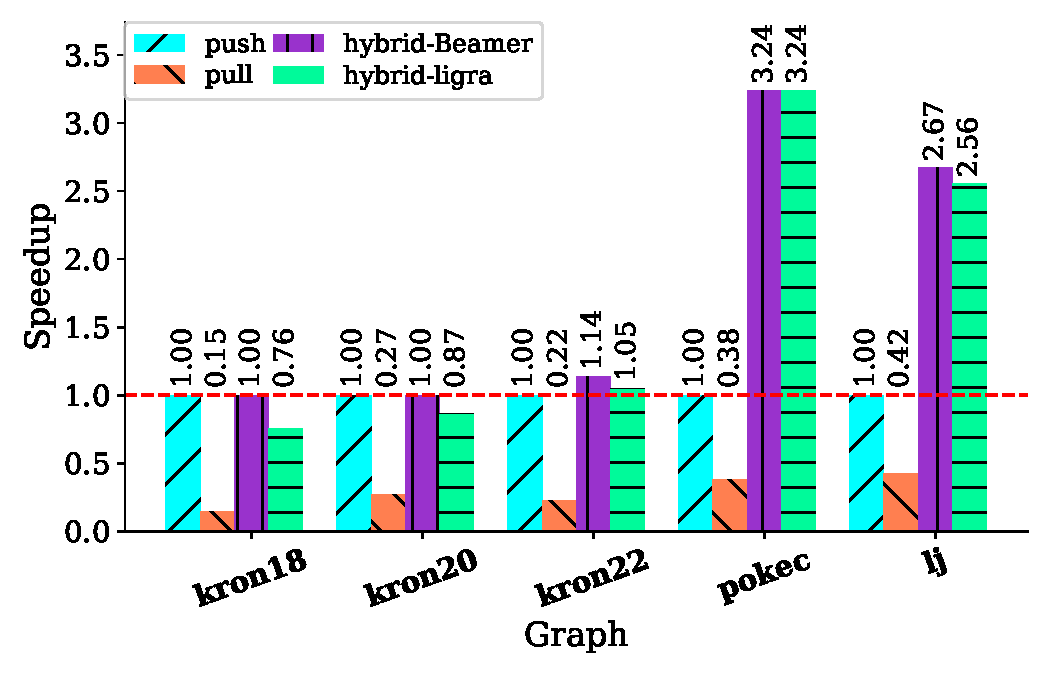
\includegraphics[scale=0.6]{graphit-figures/hybrid-dir.pdf}
    \caption{Results for different traversal methods on \hb. \todo{finish caption}}
    \label{fig:hybrid_dir}
  \end{figure}
}
%\subsection{Evaluation} \label{sec:eval}
%In this subsection, we evaluate the performance of our GraphIt code generation backend and its optimizations outlined in Sections~\ref{sec:method} and~\ref{sec:method:sub:baseline}.
%We compare the performance of our generated code to a CPU baseline and evaluate the performance of each of the optimizations we outlined in Section~\ref{sec:method}. 

\section{Experimental Setup}

%\graphInfoTable
\begin{table}[]
    %\arraystretch{1.3}
    \centering
    \begin{footnotesize}
    \begin{tabular}{lccc}
    %\hline
    \toprule
     \textbf{Name} & \textbf{Scale} & \textbf{\# Vertices} & \textbf{\# Edges} \\ \midrule %\hline
     kron18 & 18 & 262,144 & 4,194,304 \\ %\hline
     kron19 & 19 & 524,288 & 8,388,608 \\
     kron20 & 20 & 1,048,576 & 16,777,216 \\ %\hline
     kron22 & 22 & 4,194,304 & 67,108,864 \\ %\hline
     pokec (pk) & 20.5 & 1,632,803 & 30,622,564 \\ %\hline
     LiveJournal (lj) & 22 & 3,997,962 & 34,681,189 \\ %\hline
     Hollywood (hw)& 20.1 & 1,139,905 & 112,751,422 \\
     RoadCA (rc)& 20.9 & 1,971,281 & 5,533,214 \\
     RoadCent (rn)& 23.8 & 14,081,816 & 33,866,826 \\
     RoadUSA (ru)& 24.5 & 23,947,347 & 57,708,624\\
     \bottomrule
    \end{tabular}
    \end{footnotesize}
    \caption{The vertex and edge information for each of the graphs used in our evaluation. We use synthetic \kron graphs used in the Graph500 benchmark and three real world graphs.}
    \label{sec:eval:tab:graphs}
\end{table}

Host software executes natively on an Intel Xeon Gold 6254 CPU.
The host libraries interface directly with the simulator environment using the SystemVerilog DPI interface.
We compile all generated C++ code using the GNU Compiler Collection (GCC) with ``-O2''.

\paragraph{Manycore Architecture}
\tabHBParams
We evaluate our compiler using detailed RTL simulation of our manycore architecture.
We model a manycore system running at 1GHz with 16 columns and 8 rows for a total of 128 cores.
The simulation configuration details are shown in Table~\ref{tab:hbParams}.
The machine has a 512KB 8-way set associative LLC with 128-byte lines.
The memory system uses two HBM2 memory channels.
We model the HBM2 memory system with DRAMSim3\cite{li2019dramsim3},  a timing accurate simulator for modeling DRAM.
We use detailed, cycle-accurate RTL simulation to model our processor cores, network on chip, and LLC.
Our simulation environment includes SystemVerilog bind modules for collecting performance metrics such as instruction and cycle counts.
The RTL for this manycore has been validated in silicon, and this configuration occupies approximately 3.5 mm$^2$ of die area. 
%We also collect other profiling statistics such as processor stalls and opcode histograms.


\paragraph{Benchmarks} We evaluate our compiler on three common graph benchmarks: Breadth-First Search (BFS), Single Source Shortest Path (SSSP), and PageRank (PR). 
BFS has a high memory access to computation ratio and is a component of many graph algorithms.
PageRank computes the importance of each vertex in the graph, and unlike BFS, spends most of its time performing computation on the entire graph.
PR also users floating point operations.
%SSSP operates on a weighted graph.
SSSP operates on a larger subset of the edges during execution and tends to be more sensitive to load balancing.
We implement the Bellman-Ford variant of SSSP for our evaluation.

We implement all of these benchmarks in \graphit and generate manycore code using our \hb \graphvm.
Due to the time costs of simulation, we do not run all iterations of our benchmarks. 
For BFS and SSSP, we run three iterations from the middle of execution with a random root node selected as the initial frontier.
For PR, we run one iteration from the beginning of execution.



\paragraph{Graphs} We use three types of graphs in our evaluation: synthetic \kron graphs used in the Graph500 benchmark~\cite{murphy2010graph500}, real-world road networks, and real-world, social network graphs.
\kron graphs follow a power law distribution in order to simulate the small world property often seen in real world graphs~\cite{leskovec2010kronecker}.
We generate four \kron graphs of varying size. 
We primarily evaluate our results using three of these graphs: kron18, kron20, and kron22.
%We generate weighted and unweighted versions of each of these graphs for use with our three benchmarks.
We use three real-world graphs: pokec~\cite{pokec}, RoadCentral~\cite{davis2011university} and livejournal~\cite{lj}.
All of the graphs we use and their properties are shown in Table~\ref{sec:eval:tab:graphs} and discussed in more detail in Chapter~\ref{thesis:background:graphs}.


\section{Results}
%\baselineEvalFigure
\begin{figure}[h!]
    \centering
    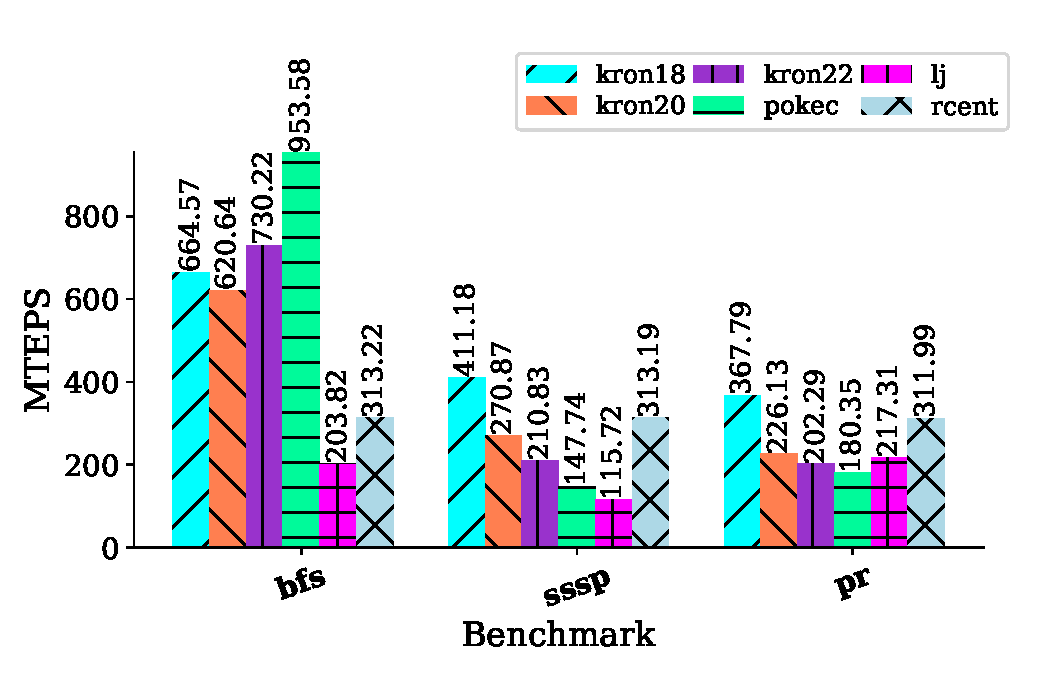
\includegraphics[scale = 0.6]{graphit-figures/baseline.pdf}
    \caption{Baseline code generation results for each benchmark in the dense pull direction with no manycore specific optimizations.}
    \label{pap:generals:sec:eval:fig:baseline}
\end{figure}

%\todo[inline]{Results intro}
To evaluate our code generator, we first present performance results for the unoptimized benchmarks. 
We then explore the performance trade-offs and benefits for each of the optimizations described in Chapter~\ref{gen:sec:optimizations}.

\subsection{Baseline}
 
%\pushEvalFigure
\begin{figure}[h!]
    \centering
    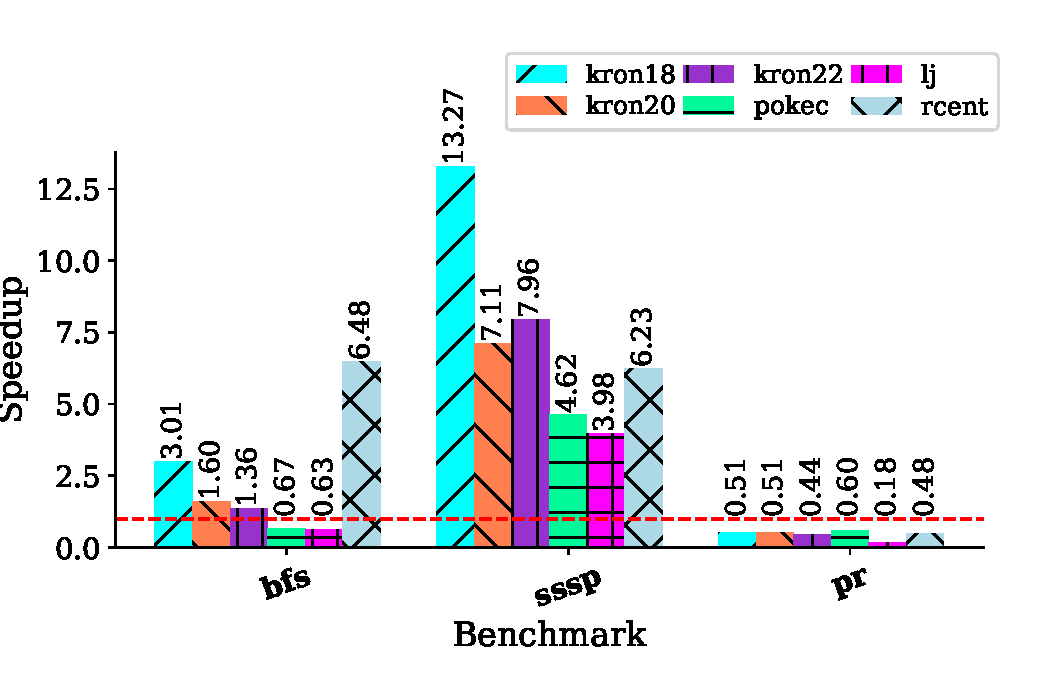
\includegraphics[scale = 0.6]{graphit-figures/push.pdf}
    \caption{Baseline code generation results for each benchmark in the push direction with no manycore specific optimizations. Speedup over the baseline pull direction is shown.}
    \label{pap:generals:sec:eval:fig:push}
\end{figure}
To establish a baseline, we examine the performance of the code produced by our backend without any added optimizations.
%To evaluate performance, we calculate the traversed edges per second (TEPS) for each iteration of each benchmark using the cycle counts that we obtain from simulation.
%We examined the performance of code produced by our backend with no added optimizations.
A key metric for our evaluation is traversed edges per second (TEPS).
We report TEPS for each iteration by counting the number of edges traversed with the applied \graphit schedule and using the cycle counts that we obtain from simulation.
This metric provide an idea of execution speed that allows for comparison between different input graphs, for which the total number of traversed edges can vary significantly.

Figure~\ref{pap:generals:sec:eval:fig:baseline} show our initial performance results for the manycore code generated by our backend without added optimizations in the \pull~direction as described in Chapter~\ref{sec:method:sub:baseline}.
%and~\ref{pap:generals:sec:eval:fig:push} show our initial performance results for the manycore code generated by our backend without added optimizations in the \pull~and \push~directions respectively as described in Section~\ref{sec:method:sub:baseline}.
Across all results, we see a geometric mean of 520.04 MTEPS in the \pull~direction.% and 104 MTEPS in the \push~direction. 
For SSSP and PR, we note that the highest performance on the \kron scale 18 graph.
This is due to the relatively small size of the graph and the large amount of parallelism and memory bandwidth of the manycore architecture.
For BFS we see the highest performance on the pokec graph.
%This decrease in performance in the \push~direction is expected as the iterations we examine for BFS and SSSP have very dense frontiers that benefit from traversing in the \pull~direction.
%In all three benchmarks, we see the highest performance on the \kron scale 18 graph.
%This is most likely due to the relative small size of the graph and the large amount of parallelism and memory bandwidth present on the manycore architecture.
 
Figure~\ref{pap:generals:sec:eval:fig:push} shows the performance of the manycore code generated in the \push direction.
Because graph traversal direction is an algorithmic optimization that changes the number of traversed edges in each iteration, we report speedup over the \pull direction in terms of total execution time here.

BFS has a very high memory access to compute ratio, so the number of reads greatly affects the performance.
We find that the \pull direction is optimal on our two real-world social-network graphs and that \push is optimal on the road-network and \kron graphs.
The two social-network graphs have a large number of edges and contain hub nodes, and as a result, these benefit most from the early termination condition in bfs \pull where visited vertices need not be examined in subsequent iterations.
%Because we use iterations from the middle of execution, a large number of vertices do not need to be visited in the \pull~direction that would need to be visited in the \push~direction. %because they have already been visited in previous iterations.
%We see an average increase in performance of 3.6$\times$ just from traversing in the \pull~direction instead of \push. 
 
Because SSSP is not able to make use of early termination in the \pull direction, the \push direction results in fewer traversed edges, and thus performs less work.
As a result, we observe speedup across all graphs when traversing in the \push direction.
From our simulation results, we also determined that the graphs made better use of LLCs in the \push direction.
 
Interestingly, the \pull~direction was optimal across all graphs on PageRank.
Unlike BFS, PageRank must visit all vertices in all iterations regardless of traversal direction.
When we examined our simulation results, we saw that the \pull~direction issued fewer read requests to HBM which most likely accounts for the performance difference.  

% We see less clear results with SSSP.
% For SSSP we observe better performance in the \pull~direction on the real world graphs, but not on the two larger \kron graphs.
% From our simulation results, we are able to see that these \kron graphs make better use of the LLCs and issue fewer reads to HBM in the \push~direction, accounting for the improvement in performance. 
 
 
 
\subsection{Blocked Access Method}


\begin{figure}[h!]
    \centering
    \subfloat[SSSP]{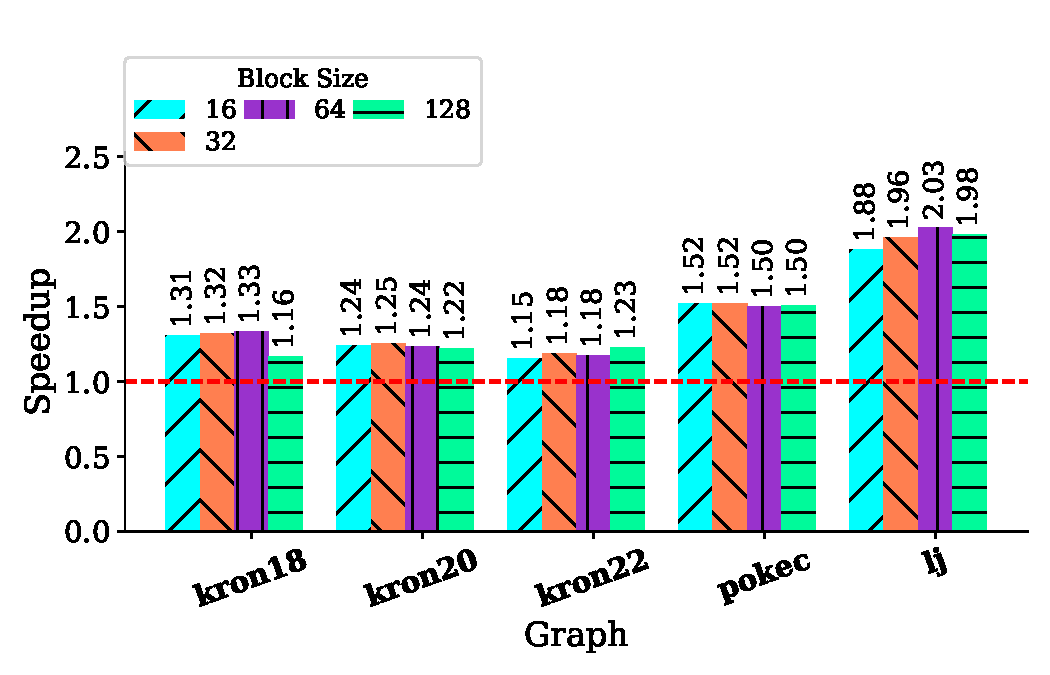
\includegraphics[scale=0.6]{graphit-figures/sssp-block.pdf}} \\
    \subfloat[BFS]{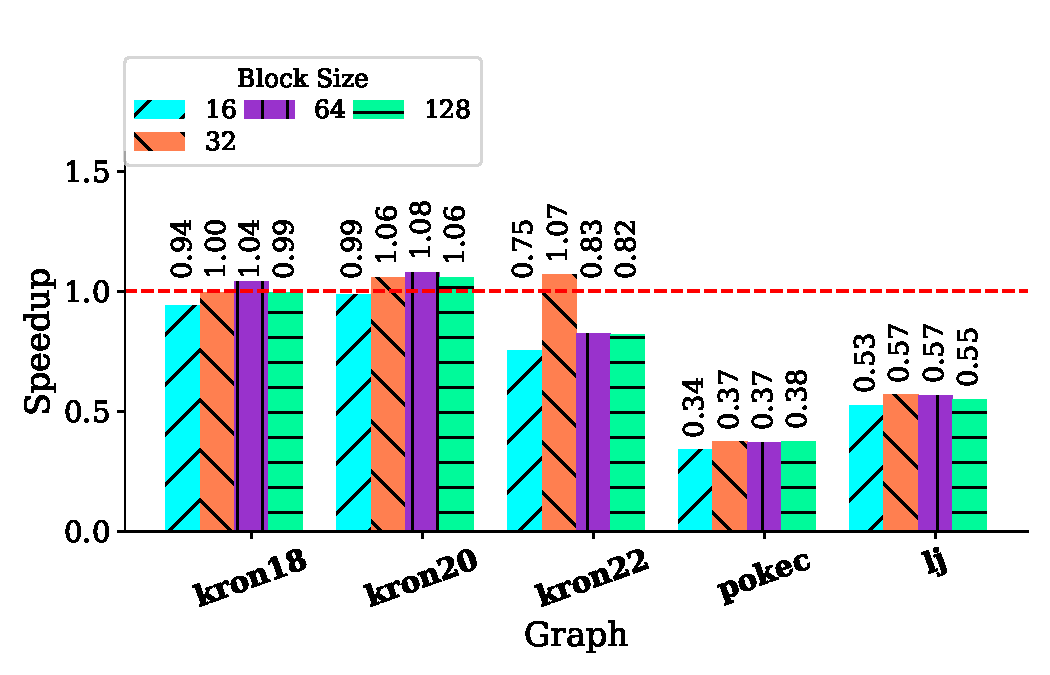
\includegraphics[scale=0.6]{graphit-figures/bfs-block.pdf}}
    \caption{Speedup results for varying block sizes using the blocked access method on BFS and SSSP. Speedup is calculated over the baseline pull direction implementation.}
    \label{pap:generals:sec:eval:fig:block}
\end{figure}
 
%\allBlockedFigure
\begin{figure}[h!]
    \centering
    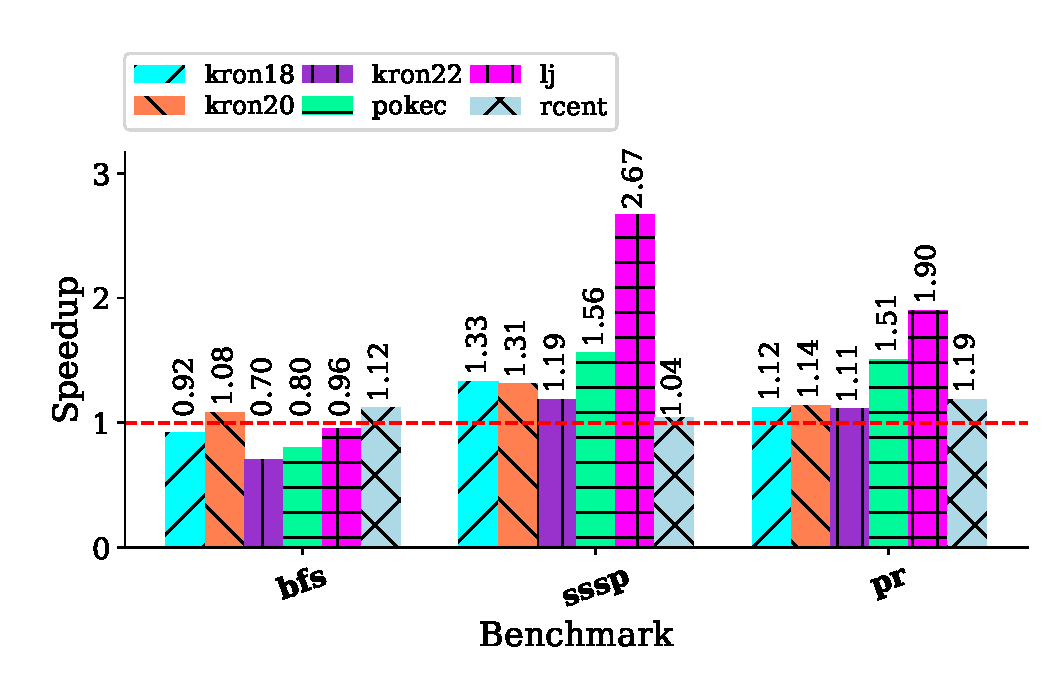
\includegraphics[scale = 0.6]{graphit-figures/all-blocked.pdf}
    \caption{Blocked access method speedup results for each benchmark. Speedup is calculated over the baseline pull direction implementation.} %For each graph and benchmark, block sizes of 16, 32, 64, and 128 elements were tested and the best performing block size is reported here.
    \label{pap:generals:sec:eval:fig:blocked}
\end{figure}
 
Figure~\ref{pap:generals:sec:eval:fig:block}a shows the performance benefit of the blocking optimization across different block sizes on the SSSP benchmark in the \pull~direction. 
Results for block sizes of 16, 32, 64, and 128 elements are shown.
Speedup is normalized to the baseline performance of SSSP in the \pull~direction without any optimizations.
Similarly, Figure~\ref{pap:generals:sec:eval:fig:block}b shows the performance benefit of the blocked access method with varying block sizes on BFS in the \pull~direction.
 
Interestingly, we do not see much variation in speedup across different block sizes. 
Livejournal and \kron 18 see the most speedup with a block size of 64, pokec and \kron 20 see optimal performance with block size 32, and a block size of 128 is optimal for \kron 22. 
We observe that the optimal block size appears to be input graph dependent for the other benchmarks we studied as well. 
 
Figure~\ref{pap:generals:sec:eval:fig:blocked} shows the speedup for each benchmark when using the blocked access method. 
Again, speedup is normalized to the baseline performance of each benchmark in the \pull~direction.
In this figure, the optimal block size for each input graph and benchmark is used to compute the speedup. 
Blocking provided a mean speedup of 1.26$\times$ and a maximum speedup of 2.67$\times$.
 
Blocking is primarily motivated by the microarchitecture's ability to hide memory load latency.
The prefetching effect from blocking can yield significant performance improvement, but it also provides the effect of data caching.
Even if the data is used once, the prefetching effect can yield significant performance improvement. 
We observe the most speedup with SSSP because it traverses more edges than BFS and benefits most from prefetching.
We see the least speedup from blocking with BFS and see performance degredation on the pokec and livejournal graphs.
The \pull~direction for BFS traverses the fewest edges of the three workloads thanks to a filter condition on destination vertices.
This means that much of the prefetched data is never used, and the additional memory reads become overhead.

Overall, we find that our blocking optimization provides performance improvement in all but four cases. 
Blocking reduces stalls from memory system requests and improves the hit rate of the LLC. 
We find, however, that it does not have a large impact on DRAM stalls.
Making use of the low-latency scratchpad memory and coalescing accesses most improve performance on benchmarks that traverse more edges in the graph. 
 
\subsection{Work Partitioning}

\begin{figure}[h!]
    \centering
    \subfloat[SSSP]{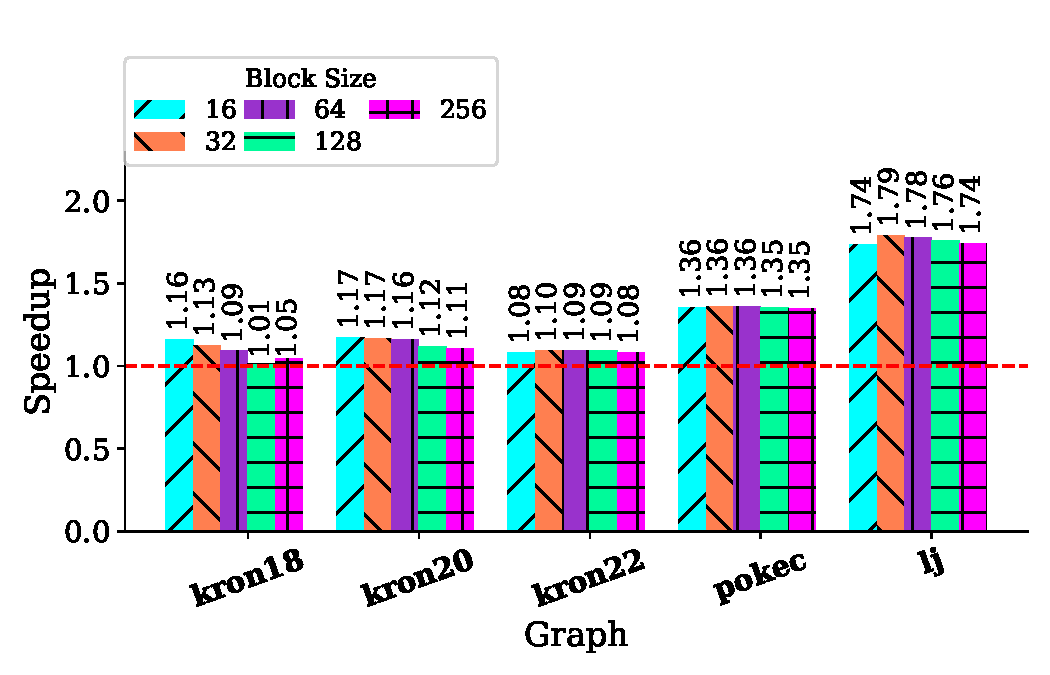
\includegraphics[scale=0.6]{graphit-figures/sssp-cache.pdf}} \\
    \subfloat[BFS]{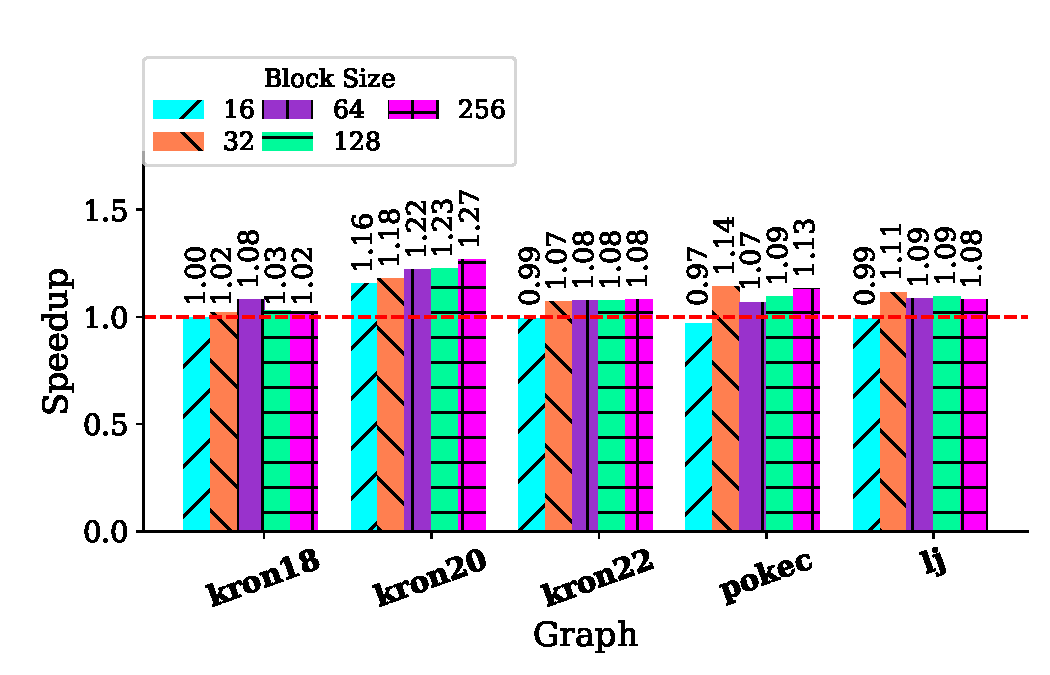
\includegraphics[scale=0.6]{graphit-figures/bfs-cache.pdf}}
    \caption{Speedup results for varying work block sizes using the manycore aware vertex partitioning scheme on SSSP and BFS. Speedup is calculated over the baseline pull direction implementation.}
    \label{pap:generals:sec:eval:fig:cache}
\end{figure}

%\allAlignedFigure
\begin{figure}[h!]
    \centering
    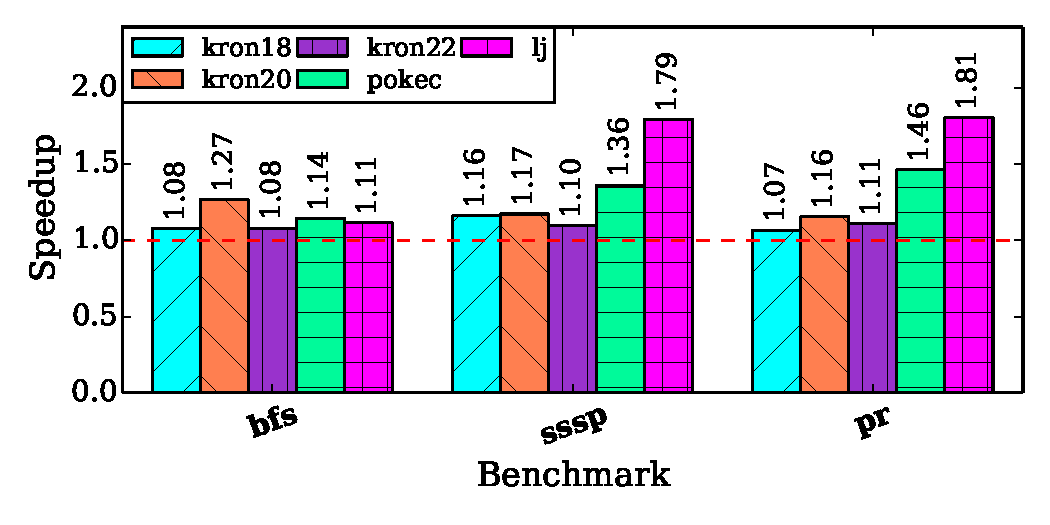
\includegraphics[scale = 0.6]{graphit-figures/align.pdf}
    \caption{Alignment-based partitioning speedup results for each benchmark. Speedup is calculated over the baseline pull direction implementation.} %For each graph and benchmark, work group sizes of 16, 32, 64, 128, and 256 vertices were tested and the best performing work group size is reported here.
    \label{pap:generals:sec:eval:fig:aligned}
\end{figure}
 
Figure~\ref{pap:generals:sec:eval:fig:cache} shows the performance benefit of alignment-based partitioning across different work block sizes on SSSP and BFS.
Speedup is calculated over the baseline SSSP \pull~implementation and baseline BFS \pull~implementation. 
Similarly to the blocked access method results, we find that the optimal work block size for alignment-based partitioning is input graph and benchmark dependent. 
%A work block size of 16 is optimal for \kron 18 and 20, livejournal and \kron22 see the best performance with a block size of 32, and pokec sees the most speedup with a block size of 64.
A work block size of 16 was optimal for \kron 18 and 20; livejournal and \kron22 saw optimal performance with a block size of 32 and pokec with a block size of 64.

Figure~\ref{pap:generals:sec:eval:fig:aligned} shows the speedup for each benchmark when using alignment-based partitioning over the baseline vertex partitioning scheme. 
The optimal work block size for each input graph and benchmark is used to calculate speedup. 
We observed a performance improvement in all input graph and benchmark combinations, with an average speedup of 1.35$\times$ and a maximum speedup of 2.68$\times$. 
 
Alignment-based partitioning aims to make better use of the memory system on the manycore. 
By assigning smaller working sets to each core, there is less contention in the LLCs and all benchmarks achieve higher cache hit rates. 
Improving the LLC hit rate decreases the total amount of memory that needs to be read from HBM and decreases the amount of time spent waiting on outstanding memory requests.
 
 
%\edgeSpeedupFigure
\begin{figure}[h!]
    \centering
    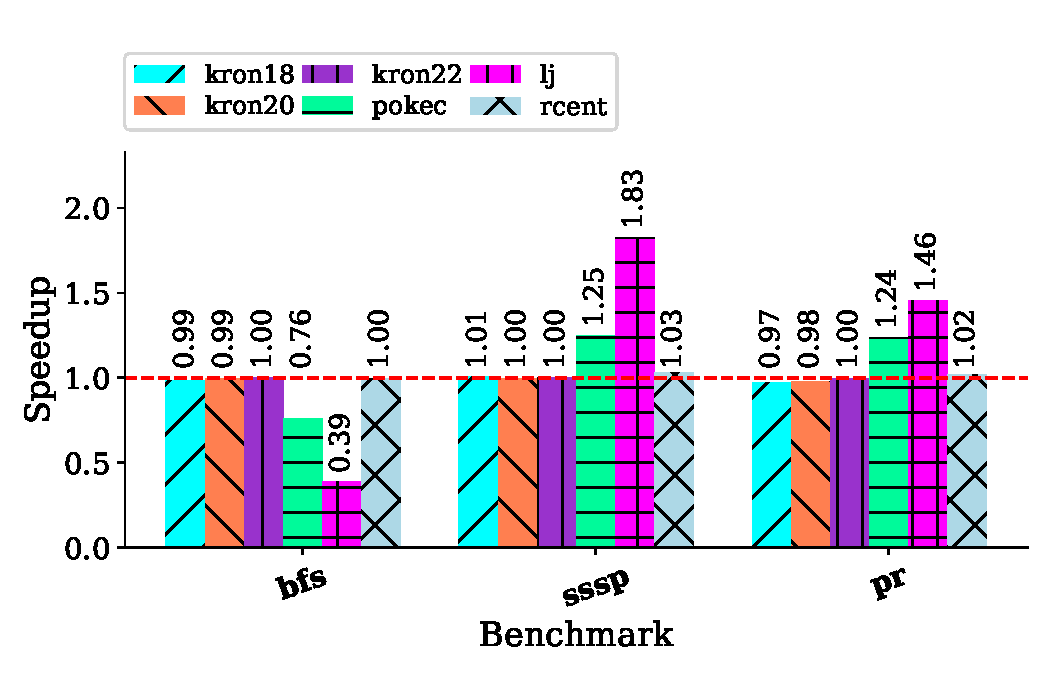
\includegraphics[scale = 0.6]{graphit-figures/edge.pdf}
    \caption{Speedup results for edge based optimization over the baseline dense pull implementation for each benchmark.}
    \label{pap:generals:sec:eval:fig:edge}
\end{figure}

\edgeAwareHist
 
Figure~\ref{pap:generals:sec:eval:fig:edge} shows the performance of edge-aware vertex partitioning relative to the baseline vertex-based partitioning on all benchmarks in the \pull~direction. 
We achieved a speedup in seven benchmarks and input graph combinations, with a maximum speedup of 1.83$\times$.
If performance degraded, we observed an average slowdown of 15.32\%. 
This scheduling optimization relies heavily on the structure of the input graph and the algorithm, so these results were somewhat expected.

Figure~\ref{fig:load_balance:cycledist} shows the core cycle count probability distribution for each benchmark on \kron graphs of scale 18, 19, and 20.
Each plot shows a probability density estimate of the total cycle counts across cores when executing both the edge-aware and vertex-based partitioning schemes for a single iteration taken from the middle of application execution.
The mean for each probability distribution is also indicated.
From this, we can see how the edge-aware work distribution affects the workload on each core.
We observe a decrease in tail latency on the edge-aware probability density curve for BFS on all input graphs in Figure~\ref{fig:load_balance:cycledist} indicating a more even load balance between cores. 

We observe a noticeable improvement in most of the SSSP experiments.
Figure~\ref{fig:load_balance:cycledist}(e) shows the most dramatic shift in terms of cycle distributions. %and Figure~\ref{fig:loadresults} showed that this scale factor achieved the best performance across the different SSSP input graphs.
PageRank sees the worst impact on cycle distribution in Figure~\ref{fig:load_balance:cycledist} when switching to the edge-aware partitioning scheme and showed slight slowdowns on kron18 and kron20 in Figure~\ref{pap:generals:sec:eval:fig:edge}.
These results show that the edge-aware scheme does have a noticeable impact on cycle count and load balancing
 
Overall, while we see performance improvements with edge-aware vertex-based partitioning on some benchmarks, we find that alignment-based partitioning provides the most performance improvement in all cases. 
Despite its workload balancing benefits, edge-aware partitioning does not account for the manycore specific properties of the memory system.
Because the memory is the main bottleneck of graph algorithms, the alignment-based scheme which explicitly takes into consideration the properties of the manycore's memory system is ideal. 

\subsection{Bucketed Sparse Frontier}

\begin{figure}[h!]
    \centering
    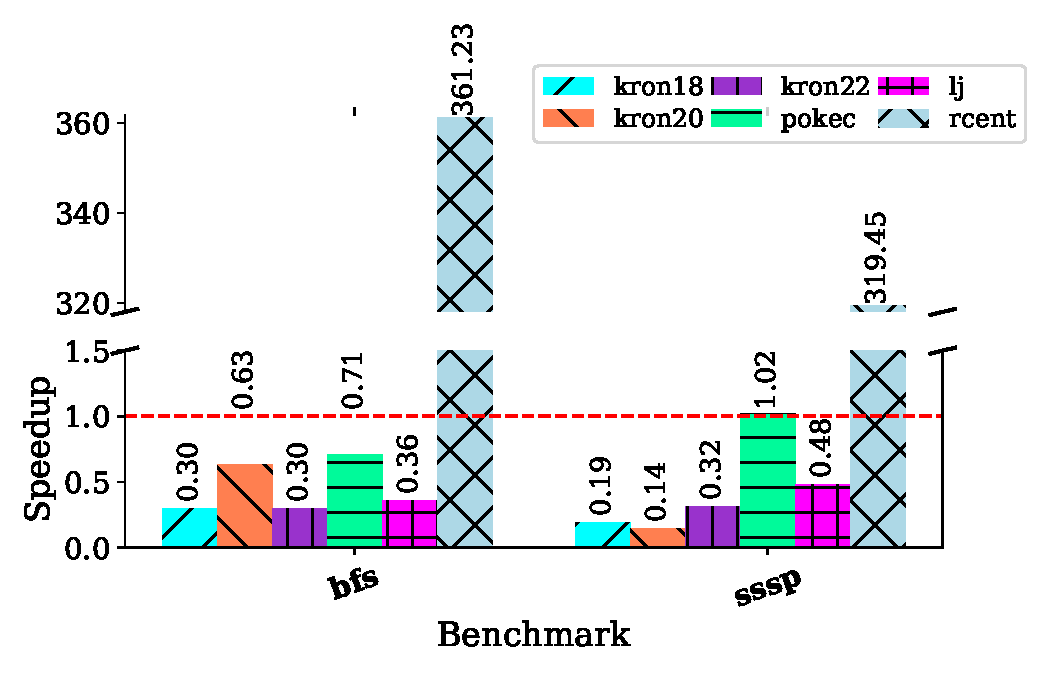
\includegraphics[scale=0.6]{graphit-figures/sparse.pdf}
    \caption{Bucketed sparse frontier speedup results for each benchmark. Speedup is calculated over the baseline \push direction implementation.} %For each graph and benchmark, work group sizes of 16, 32, 64, 128, and 256 vertices were tested and the best performing work group size is reported here.
    \label{pap:cgo2020:sec:eval:fig:sparse}
\end{figure}

Figure~\ref{pap:cgo2020:sec:eval:fig:sparse} shows the performance of the bucketed sparse frontier optimization relative to the baseline vertex-based partitioning for all benchmarks in the \push direction.
We only evaluate this optimization on BFS and SSSP because PR is not a frontier based algorithm.
We find the largest improvement on the road\_central graph with a speedup of 361.23$\times$ for BFS and 319.45$\times$ for SSSP.
This is expected as it has the smallest frontiers and vertices in the graph have very low degree, and thus benefits the most from removing unnecessary reads to the frontier.

We observed a large slow down in almost every other case.
This was due to an increase in cache line contention that decreased the LLC hit rate. 
Cores ended up issuing more read requests concurrently with this scheme than they did using a dense frontier which degraded performance.

\subsection{Hybrid Traversal}
\alphatune
\betatune
To evaluate hybrid traversal on \hb, we first tune the $\alpha$ and $\beta$ variables used in the heuristics proposed by Beamer et al.
Figure~\ref{fig:alpha_tuning} shows the results for tuning $\alpha$ to the \hb~manycore on 5 different input graphs. 
We run BFS without optimizations for 10 iterations on each graph.
We don't evaluate on any road networks as these graphs rarely benefit from hybrid traversal.
We examine values of $\alpha$ between 1 and 30.
While Beamer et al. found $\alpha=15$ to be optimal on an Intel IvyBridge server, we find that the optimal value of $\alpha$ is much lower.
For BFS with the graphs we studied, we find that $\alpha=5$ provides the best performance in the most cases.

The results for tuning $\beta$ are shown in Figure~\ref{fig:beta_tuning}.
Again, we run BFS for 10 iterations on the same input graphs.
We choose values for $\beta$ in the range 1 to 1024.
Again, the optimal $\beta$ value for \hb is lower than the one found by Beamer et al.
We find $\beta=4$ to provide the best performance in the most cases.

Our lower $\alpha$ and $\beta$ values result in hybrid traversal preferring the \push direction.
Repeating this study with alignment-based partitioning in the \pull direction or repeating it for different benchmarks might yield slightly higher $\alpha$ and $\beta$ values.
However, the differences in the memory hierarchies between an Intel IvyBridge server and the \hb~manycore likely account for the lower values.

\hybridresults
Finally, we present results for \push, \pull, Beamer's hybrid traversal (with $\alpha=5$ and $\beta=4$), and Ligra's hybrid traversal in Figure~\ref{fig:hybrid_dir}.
We evaluate 10 iterations of BFS with the same input graphs. 
We report speedup relative to the \push implementation results.
Similarly to Figure~\ref{pap:generals:sec:eval:fig:push}, we find that traversing in the \pull direction results in a slowdown over \push on the \kron graphs. 
Because we sample a larger number of iterations here, we also observe a slowdown for \pull on Livejournal and pokec. 
With the values of $\alpha$ and $\beta$ that we use, we find that Beamer's hybrid traversal never switches to \pull on kron18 and kron20. 
For these graphs we see a performance decrease with the Ligra hybrid traversal method.
On the two real-world graphs, we see larger performance improvements up to $3.24\times$.
We also find that Ligra's hybrid traversal is able to achieve performance within $4.5\%$ of the performance of Beamer's hybrid traversal implementation on the two real-world graphs and is within $12\%$ on average across all graphs studied.
Because of this and because of the simplicity of its implementation, we use the Ligra hybrid traversal heuristic in our runtime libraries.
 
\subsection{Performance Analysis}

\begin{figure}[h]
    \centering
    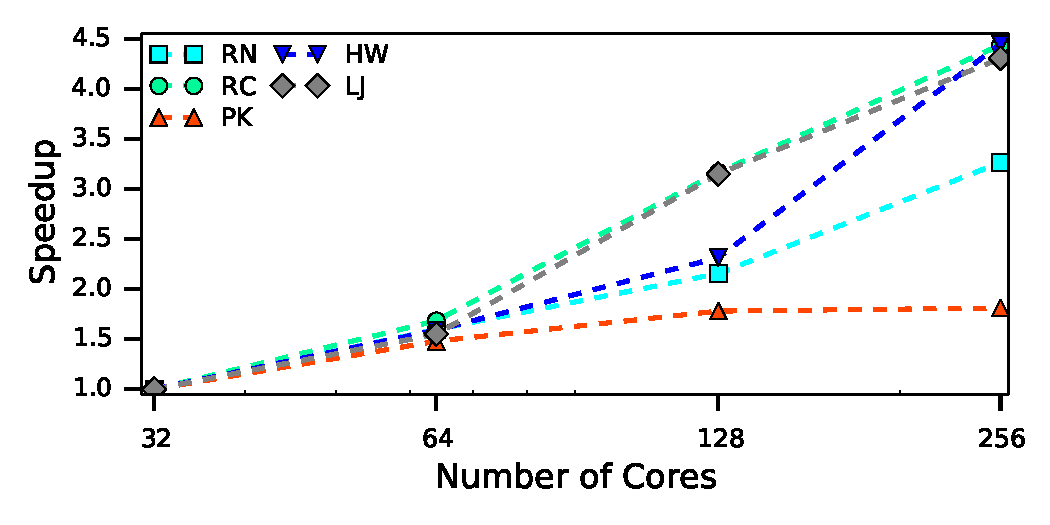
\includegraphics[scale = 0.6]{graphit-figures/hb-scaling-speedup.pdf}
    \caption{Scaling results for BFS across four \hb~manycore configurations. LLC capacity and the number of columns (16) is held constant while the number of rows is varied from 2 to 16.} 
    \label{pap:generals:sec:eval:fig:scaling}
\end{figure}

\hbBlockingEvalTab

Figure~\ref{pap:generals:sec:eval:fig:scaling} shows how performance scales on the \hb~manycore as the number of cores are varied.
Optimized BFS code was executed on four different machine configurations: we hold the LLC capacity and number of columns (16) constant
and vary the number of rows (2, 4, 8, and 16) to vary the total number of cores.
We observe increased performance as we increase the number of cores, suggesting that the generated code provides sufficient parallelism to obtain high performance.
The strong scaling indicates that our generated code can successfully exploit parallelism.
We highlight BFS for this scaling study due to its high memory access to compute ratio.
Because memory is a major bottleneck for most graph applications, we anticipate that these scaling trends will continue to hold for other applications. 

Table~\ref{tab:hb_blocking} demonstrates performance improvements for SSSP with delta-stepping when the blocked-access optimization is applied on three selected input graphs.
The table shows the overall performance speedup, the improvement in effective random access bandwidth, and the reduction in DRAM stalls during execution for the three input graphs where the this optimization was applied.
The blocked-access optimization loads fixed-size blocks of vertex data into local scratchpad memory.
Loading the data into scratchpad reduces access latency in exchange for bandwidth.
This optimization exploits memory parallelism to hide DRAM access latency in exchange for loading unused data and reducing effective bandwidth.
%We observe that DRAM stalls decrease and memory bandwidth utilization increases substantially for all three input graphs.
For SSSP, we observe that this optimization decreases DRAM stalls, increases memory bandwidth utilization, and improves overall application performance.
Because SSSP is a data driven application, it benefits from this optimization which targets the memory hierarchy and utilizes the manycore's software managed scratchpads.

